\section{Ergebnisse}
\label{sec:ergebnisse}
In diesem Abschnitt werden die Ergebnisse der Datenauswertung wiedergegeben und interpretiert.
Die Auswertungen der verschiedenen Studien haben gezeigt, dass Code-Metriken mit Sicherheitslücken auf statistisch signifikanten Niveau\cite{chowdhury_zulkernine_2010,chowdhury_zulkernine_2009,alves_et_al}.

Chowdhury und Zulkernine \cite{chowdhury_zulkernine_2010} zeigen, dass die CCC-Metriken im Durchschnitt eine Korrelation von 0.5 aufweisen mit einem p-Wert < 0.05.
Dies bestätigt die erste Hypothese auf Abschnitt \ref{sec:hypothesen}.
\begin{figure}
	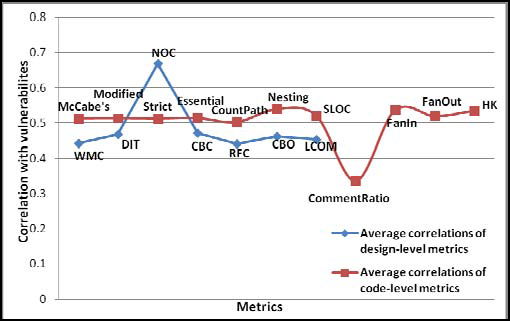
\includegraphics[width=\textwidth]{img/code_vs_design.png}
	\label{fig:code_vs_design}
	\caption{Durchschnittliche Korrelation mit Sicherheitslücken für gegebene Metriken; Einteilung nach Code-Level und Design-Level}
\end{figure}
Abbildung \ref{fig:code_vs_design} zeigt, inwieweit die einzelnen Metriken von der durchschnittlichen Korrelation der jeweiligen Gruppe (Code-Level bzw. Design-Level) abweichen.
Es konnte festgestellt werden, dass die Anzahl der Unterklassen ("`Number of Children"') die höchste Korrelation mit Sicherheitslücken aufweist, während das Verhältnis von Kommentaren zu Quellcode nur schwach korreliert.
Zusätzlich konnte festgestellt werden, dass die Verteilung der Korrelationen über mehrere Versionen von Mozilla Firefox hinweg konsistent ist.

Alves \emph{et al} \cite{alves_et_al} machen mit ihrer Forschung diese Ergebnisse repräsentativer, indem sie eine ähnliche Codeanalyse an fünf Projekten mit insgesamt 2875 geschlossenen Sicherheitslücken durchführen.
Die Ergebnisse bestätigen, dass statistisch signifikante Korrelationen zwischen den Metriken und vorhandenen Sicherheitslücken herrschen.
Die Forschung konnte nicht bestätigen, dass sich durch die Metriken die Anzahl der Sicherheitslücken ermitteln lässt.
Demnach kann die zweite Hypothese aus \ref{sec:hypothesen} nicht bestätigt werden.
Es wird auch gezeigt, dass das Verhältnis von Kommentaren zu Quellcode höher in Code mit Schwachstellen ist.
Nicht-betroffener Code zeigt in den meisten Fällen gar keine Kommentare auf.

Medeiros \emph{et al} \cite{medeiros_et_al} verwenden den gleichen Datensatz von wie Alves \emph{et al} \cite{alves_et_al} um zu untersuchen, wie die Metriken untereinander in Korrelation stehen und welche sich am besten für die Vorhersage von Sicherheitslücken eignet.
Ihre Ergebnisse zeigen, dass einige der Metriken auf Projektebene miteinander korrelieren.
Es kann festgestellt werden, dass die Wahl der geeigneten Metriken für die Vorhersage projektabhängig ist.
Die Forscher stellen fest, dass Code-Metriken auf verschiedenen Ebenen (Funktions-, Datei- und Projektebene) komplementär zueinander sind und durch die Kombination bessere Ergebnisse bei der Vorhersage erzielt werden können.
Die dritte Hypothese aus \ref{sec:hypothesen} kann bestätigt werden.

In \cite{chowdhury_zulkernine_2009} erweitern Chowdhury und Zulkernine ihre Forschung von \cite{chowdhury_zulkernine_2010} und verwenden durch Maschinelles Lernen generierte Klassifikatoren, um ein Framework für die Entdeckung von Sicherheitslücken zu entwickeln.
Das erstellte Framework kann die Mehrzahl der Dateien mit Sicherheitslücken in Mozilla Firefox erkennen.
Es zeigt auch, dass die historischen Informationen des Projektes verwendet werden können, um künftige Sicherheitslücken zu finden.
Dafür haben die Forscher von den 52 vorhandenen Versionen von Mozilla Firefox 32 zum Training der Klassifikatoren verwenden und die restlichen 20 zum Testen.
Es ist anzumerken, dass die Ergebnisse der historischen Untersuchung weniger gut waren.
